\begin{frame}{ Outline}
  \begin{itemize}
  \item \textcolor{gray}{Background: Core Model and Implementation}
    \air
  \item \textcolor{gray}{Work 1: Generation  }
    \air

  \item \textbf{Work 2: Attention (\textit{Latent Alignment and Variational Attention})}
    \air


  \item \textcolor{gray}{Challenges: Text Generation and Deep Learning}
  \end{itemize}

  \begin{center}
    \textbf{Can we learn to control what facts are used?}
  \end{center}
\end{frame}


\begin{frame}{Machine Learning for Text Generation: Translation}
  \begin{center}
    \begin{tikzpicture}

      \node (gal) {\includegraphics[width=1.5cm]{phone}};
      \node [rounded corners, above =(0.2cm) of gal] {$p_{\theta}$};

      \node (a) [rectangle, yshift=1cm, xshift=-5cm, scale=0.8, draw,thick,fill=blue!0,text width=16em, rounded corners, inner sep =5pt, minimum height=1em] {
        Yalitza Aparicio acababa de graduarse de una escuela para maestros y aun no tenia empleo cuando el proceso de busqueda de actrices para la ultima pelicula de Alfonso Cuaron llego a su natal Tlaxiaco, Oaxaca.
};
      \path[draw, ->] (a) --  (a -|  gal.west) ;


      \node [rounded corners, above =(0.2cm) of a] {$x$};

      \visible{
        \node(b) [xshift=4.5cm, yshift=-1cm, rectangle, scale=0.8, draw,thick,fill=blue!0,text width=12em, rounded corners, inner sep =5pt, minimum height=1em]{\baselineskip=50pt \small
          Yalitza Aparicio had just finished her teaching degree and didn't yet have a job when the Mexican director Alfonso Cuaron held a casting call in her home of Tlaxiaco, Oaxaca, for the lead role in his semi-autobiographical drama, ``Roma.''

          \par};

        \node [rounded corners, above = (0.2cm) of b] {$y_{1:T}$};
        \path[draw, <-] (b) --  (b -| gal.east) ;
      }
    \end{tikzpicture}
  \end{center}
\end{frame}

% \begin{frame}
% { Six Challenges for NMT (Koehn and Knowles 2017)}
% \begin{itemize}
%     \item \textbf{2: Requires large sample complexity}
%     \air
%     \item \textbf{5: The alignments learned by soft attention may not
%         be interpreted as word alignments}
%     \air
% \end{itemize}
% \end{frame}



\begin{frame}{Latent-Variable Alignment Model}
  \begin{center}


  \begin{tikzpicture}[every node/.style={anchor=base,minimum size=8mm}]
    \matrix  (graph) [matrix of nodes, row sep=0.5em,column sep=-0.3em,
    minimum width=0.2em, minimum height=0.5em, font=\small,ampersand replacement=\&] {
      \phantom{M}Mary\phantom{p} \&
      \phantom{M}did\phantom{p} \&
      \phantom{M}not\phantom{p} \&
      \phantom{M}slap\phantom{p} \&
      \phantom{M}the\phantom{p} \&
      \phantom{M}green\phantom{p} \&
      \phantom{M}witch\phantom{p} \\
      $z$ \& \& \& \& \& \& $\substack{\textcolor{blue}{p(y, z | x)} \\ \textcolor{red}{} }$ \\
      Maria \&
      no \&
      \textbf{daba} \&
      una \&
      bofetada \; a\&
       la \; bruja \&
      verda\\
    };


    \begin{scope}[on background layer]
      \draw[] (graph-1-1.south) -- (graph-3-3.north);
      \draw[] (graph-1-2.south) -- (graph-3-3.north);
      \draw[] (graph-1-3.south) -- (graph-3-3.north);
      \draw[] (graph-1-4.south) -- (graph-3-3.north);
      \draw[] (graph-1-5.south) -- (graph-3-3.north);
      \draw[] (graph-1-6.south) -- (graph-3-3.north);
      \draw[] (graph-1-7.south) -- (graph-3-3.north);

      % \draw[draw=red!30, line width=0.2mm] ($(graph-1-1) + (0.1, 0)$) -- ($(graph-3-3) + (0.1, 0)$);
      % \draw[draw=red!30, line width=0.2mm] ($(graph-1-2) + (0.1, 0)$) -- ($(graph-3-3) + (0.1, 0)$);
      % \draw[draw=red!30, line width=0.1mm] ($(graph-1-3) + (0.1, 0)$) -- ($(graph-3-3) + (0.1, 0)$);
      % \draw[draw=red!30, line width=0.9mm] ($(graph-1-4) + (0.1, 0)$) -- ($(graph-3-3) + (0.1, 0)$);
      % \draw[draw=red!30, line width=0.1mm] ($(graph-1-5) + (0.1, 0)$) -- ($(graph-3-3) + (0.1, 0)$);
      % \draw[draw=red!30, line width=0.4mm] ($(graph-1-6) + (0.1, 0)$) -- ($(graph-3-3) + (0.1, 0)$);
      % \draw[draw=red!30, line width=0.1mm] ($(graph-1-7) + (0.1, 0)$) -- ($(graph-3-3) + (0.1, 0)$);

      \draw[rounded corners, fill=green!10] ($ (graph-1-1.north west) -(-0.1,0.1)$) rectangle  node[yshift=0.8cm]{\textcolor{red}{}} ($(graph-1-1.south east) -(0.1,-0.1)$ ) ;
      \draw[rounded corners, fill=red!10] ($ (graph-1-2.north west) -(-0.1,0.1)$) rectangle  node[yshift=0.8cm]{\textcolor{red}{}} ($(graph-1-2.south east) -(0.1,-0.1)$ ) ;
      \draw[rounded corners, fill=blue!10] ($ (graph-1-3.north west) -(-0.1,0.1)$) rectangle  node[yshift=0.8cm]{\textcolor{red}{}} ($(graph-1-3.south east) -(0.1,-0.1)$ ) ;
      \draw[rounded corners, fill=orange!10] ($ (graph-1-4.north west) -(-0.1,0.1)$) rectangle  node[yshift=0.8cm]{\textcolor{red}{}} ($(graph-1-4.south east) -(0.1,-0.1)$ ) ;
      \draw[rounded corners, fill=black!10] ($ (graph-1-5.north west) -(-0.1,0.1)$) rectangle  node[yshift=0.8cm]{\textcolor{red}{}} ($(graph-1-5.south east) -(0.1,-0.1)$ ) ;
            \draw[rounded corners, fill=purple!10] ($ (graph-1-6.north west) -(-0.1,0.1)$) rectangle  node[yshift=0.8cm]{\textcolor{red}{}} ($(graph-1-6.south east) -(0.1,-0.1)$ ) ;      \draw[rounded corners, fill=brown!10] ($ (graph-1-7.north west) -(-0.1,0.1)$) rectangle  node[yshift=0.8cm]{\textcolor{red}{}} ($(graph-1-7.south east) -(0.1,-0.1)$ ) ;

      \draw[rounded corners] ($ (graph-3-1.north west) +(-0.1,0.1)$) rectangle  node[yshift=-0.8cm]{\textcolor{red}{}} ($(graph-3-7.south east) +(0.1,-0.1)$ ) ;

      \draw[rounded corners] ($ (graph-1-1.north west) +(-0.1,0.1)$) rectangle  node[yshift=0.8cm]{\textcolor{red}{}} ($(graph-1-7.south east) +(0.1,-0.1)$ ) ;

      % \draw[rounded corners,fill=green!10] (graph-1-1.north west) rectangle  node[ yshift =0.7cm] {$x_{1:T}$} (graph-1-7.south east);

      \path[] (graph-3-3.north west) rectangle  node[yshift=-0.9cm]{\textbf{$y_3$}} (graph-3-3.south east);

      % \draw[rounded corners, fill=blue!10] (graph-3-1.north west) rectangle  node[yshift=-0.9cm]{\textcolor{blue}{$$}}  ($(graph-3-2.south east) + (-0.1, 0)$);

    \end{scope}
  \end{tikzpicture}
  \end{center}
\end{frame}






% \begin{frame}
% {This Work: A Study of Attention Models}
%      General method with many applications in,
%     \begin{enumerate}
%         \item \textbf{Translation}
%         \item Speech Recognition
%         \item Summarization
%         \item Image Generation
%     \end{enumerate}
%     \air

% \begin{itemize}
%     \item Can they be improved?
%     \item Can we incorporate external information?
%     \item Can we build in inductive bias?
% \end{itemize}
% \end{frame}

% \section{Formal Description}
% \begin{frame}
%   \begin{center}
%     \textbf{Seq2Seq+} \air

%   \end{center}
% \center
% \vspace{-5mm}
%  \air
% \includegraphics[scale=0.37]{nmt-attn3}
% \end{frame}

% \begin{frame}{Notation: Alignment Model}
% \begin{itemize}
%     \item $x$ = $x_1,\cdots, x_T$: the observed source words
%     % \item $\tilde{x}$: the query (the decoder hidden state at a single timestep)
%     \item $y$: the output (the current target word)
%     \item $z$: the latent alignment, random variable indicating which member of $x$ generates $y$
% \air
% \end{itemize}
% \end{frame}


% \begin{frame}{Neural Attention versus Latent Alignment}
% \begin{itemize}
%      \item Attention is motivated as an approximation to alignment:
%         \begin{itemize}
%             \item makes the model's behavior interpretable
%             \item can be used for other prediction tasks
%         \end{itemize}
%     \air
%     % \item Soft Attention is \textit{deterministic}  from a neural network,
%     \air

%     % \item We contrast this with latent alignment which acts as a random variable.
%     %   \air

%     \end{itemize}
%     \centerline{\textbf{Key Distinction}}
%     \begin{itemize}
%     \item Both can compute $p(x | z)$ but attention cannot compute
%       posterior $p(z | x)$.
%     \end{itemize}
% \end{frame}


\begin{frame}{Latent Alignment: Motivation}

If attention works so well, why study alignment?

\begin{itemize}
    \item A latent variable approach  facilitates \structure{composibility}  in a principled probabilistic manner. (Cohn et al, 2016)
    \air
    \item \structure{Posterior inference} provides better post-hoc interpretability and analysis
    \air
    \item Modeling \structure{uncertainties} might lead to better performance
\end{itemize}
\end{frame}

\begin{frame}
  {Concurrent Experimental Work}

  Many different researchers have recently explored the
  benefits of marginalization. Very similar results.

  \begin{itemize}
  \item Surprisingly Easy Hard-Attention for Sequence to Sequence Learning
  \item Hard Non-Monotonic Attention for Character-Level Transduction
  \item Posterior Attention Models for Sequence to Sequence Learning
  \item ...
  \end{itemize}
\end{frame}

\begin{frame}{Problem Setup}
\begin{itemize}
\item Let $a$ be the prior alignment distribution of $z$
\item Let $f(x,z;\theta)$ be the likelihood of $y$ given $z$
    \begin{eqnarray*}
        z \sim a(x;\theta ) \ \ \ \  y \sim f(x, z; \theta)
    \end{eqnarray*}
\item Training Objective (maximizing marginal log-likelihood)
    \begin{eqnarray*}
        {\cal L}(\theta) =  \log \sum_z p(y = \hat{y}, z \given  x) &=&  \ \log \E_z [f(x, z;\theta)_{\hat{y}}]
    \end{eqnarray*}

\begin{figure}
\centering
\begin{tikzpicture}
\node(z)[latent]{$z$};
\node(y)[right =of z, latent]{$y$};
\node(x)[obs, above = of y]{$x$};
%\node(xp)[above= of z, obs]{$\tilde{x}$};
% \plate {} {(x)} {};
\edge {x} {y};
%\edge {xp} {z};
\edge {x} {z};
\edge {x} {y};
\edge {z} {y};
\end{tikzpicture}
\end{figure}


%     \begin{itemize}
%         \item Discrete $z\sim{\mcD}$: $O(T)$ additional runtime
%         \item Continuous ${z\sim\mcD}$: intractable
%     \end{itemize}
\end{itemize}
\end{frame}


\begin{frame}{Key Issue: Computational Cost}

  \begin{itemize}
  \item Direct optimization is computationally expensive
    \[  \ \log \E_z [f(x, z;\theta)_{\hat{y}}]\]


  \item Computing expectation requires summing over source for each target.
    \air

  \item Translation bottlenecked by training scale.
  \end{itemize}

\end{frame}

\begin{frame}{Workaround 1: Soft Attention}
\begin{itemize}
\item Replace the joint distribution with a nested expectation
{\small[Bahdanau et al 2014]}
    \begin{eqnarray*}
        \log \E_z [f(x, z)_{\hat{y}}] \approx \log f(x,\E_z[z])_{\tilde{y}}
    \end{eqnarray*}
\item The corresponding graphical model is
\air
\begin{figure}
        \centering
        \begin{tikzpicture}
            \node(y)[latent]{$y$};
            \node(x)[obs, above = of y]{$x$};
            % \node(xp)[left= of x, obs]{$\tilde{x}$};
            % \plate {} {(x)} {};
            % \edge {xp} {y};
            \edge {x} {y};
        \end{tikzpicture}
    \end{figure}
\end{itemize}
\end{frame}

\begin{frame}{Soft Attention}
%   \begin{center}
%     \textbf{Seq2Seq+} \air

%   \end{center}
% \center
% \vspace{-5mm}
%  \air
  \begin{center}
\includegraphics[scale=0.37]{nmt-attn4}
\end{center}
\end{frame}


\begin{frame}{Workaround 2: Hard Attention}
\begin{itemize}
% \item Keep the latent variable model formulation and maximize a lower bound
% on the marginal likelihood
% \air
\item {\small[Xu et al 2015]}: Directly apply Jensen's inequality and optimize
    with REINFORCE by sampling from the prior
    \begin{eqnarray*}
        \log \E_z [f(x, z)_{\hat{y}}] \ge \E_z \log [f(x, z)_{\hat{y}}] \approx \log f(x, \tilde{z})_{\hat{y}}
    \end{eqnarray*}


  \item Problems:
    \begin{itemize}
    \item The use of the prior in the expectation may result in a poor
      bound
    \item Cannot directly use for posterior estimation $p(z\ |\ y, x)$
    \end{itemize}
  \end{itemize}
\end{frame}


\begin{frame}
{Marginal Likelihood: Variational Decomposition}

For any$^*$
% \footnote{Technical condition: $\text{supp}(q(z)) \subset \text{supp}(p(z \given x ; \theta))$}
distribution $q(z)$ over $z$,
\begin{align*}
 L(\theta) &= \textcolor{red}{\E_{q}\Big[\log p(y \given x, z) \Big] - \KL[q(z) \, \Vert \, p(z
  \given x)] } \\ &
+ \textcolor{blue}{\KL[q(z )  \, \Vert \, p(z \given y, x )]}
\end{align*}

\begin{center}
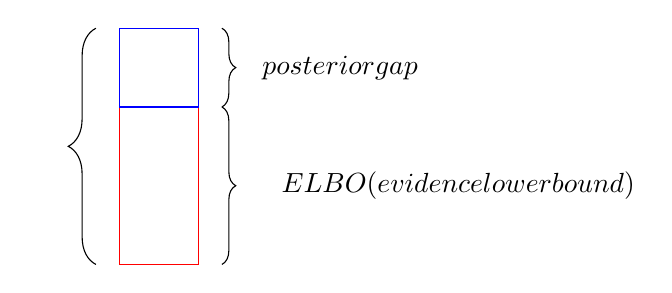
\begin{tikzpicture}
    \draw[decorate,decoration={brace,amplitude=10pt}] (-0.3, 0) -- node[xshift=-0.75cm]{} (-0.3, 3);

    \draw[red] (0, 0) rectangle (1, 2);
    \draw[blue] (0, 2) rectangle (1, 3);
    \draw[decorate,decoration={brace,amplitude=5pt}] (1.3, 2) -- node[xshift=3cm]{$\alert{\text{ELBO  (evidence lower bound) }}$} (1.3, 0);
    \draw[decorate,decoration={brace,amplitude=5pt}] (1.3, 3) -- node[xshift=1.5cm]{$\structure{\text{posterior gap}}$} (1.3, 2);
\end{tikzpicture}
\end{center}

%\begin{itemize}
%    \item The \alert{evidence lower bound} (ELBO)
%    \item The \structure{posterior gap}
%\end{itemize}

Since KL is always non-negative, $L(\theta) \geq \text{ELBO}(\theta, \lambda)$.
\end{frame}


\begin{frame}{Variational Attention}
\begin{itemize}
    % \item Note that we must have $\textrm{supp } q(z) \subseteq \textrm{supp } p(z \given x, \tilde{x}, y)$
    \item Learn model and $q$ to maximize the following lower bound
        \begin{align*}
        \log &\E_{z \sim p(z \given x,)}[p(y \given x, z)]\\
        &\ge\E_{z \sim q(z)}[\log p(y \given x, z)] - \KL[q(z) \, \Vert \, p(z
  \given x)]
        \end{align*}
    \item We choose a $q(z)$ that affords analytic KL
    \item At test time, marginalize over $z$.
\end{itemize}
\end{frame}


\begin{frame}
{Example Form of $q$: Amortized Parameterization}
\begin{center}
    \begin{tikzpicture}
% nodes
 \node[latent] (zl) {$z$};%
  \node[below=of zl] (xl) {};%
 \node[obs, right=of xl] (xtilde) {$x$};%
 \node[obs, left=of xl] (yl) {$y$};%
 %\node[obs, right=1cm of dots] (xT) {$x_T^{(n)}$};%
 \node[const, above=of zl] (lambda) {$\lambda$};
% plate
 \edge{lambda}{zl};
 \edge{yl}{zl};
 % \edge{xl}{zl};
\edge {xtilde} {z};
% \plate {} {(xtilde)} {};

 \begin{scope}[xshift=5cm]
\node(z)[latent]{$z$};
\node(y)[right =of z, latent]{$y$};
\node(x)[obs, above = of y]{$x$};
% \node(xp)[above= of z, obs]{$\tilde{x}$};
% \plate {} {(x)} {};
\edge {x} {y};
% \edge {xp} {z};
\edge {x} {z};

\edge {x} {y};
\edge {z} {y};
 \end{scope}
 \draw[dashed] (zl) --node [yshift=0.2cm] {$\KL(q(z) || p(z \given x,  y))$} (z);
\end{tikzpicture}
\end{center}
$\lambda$ parameterizes a global network (encoder) that is run over $x, y$
    to produce the local variational distribution, e.g.
    \[ q(z ; \lambda) = \text{enc}(x,  y ; \lambda)\]
\end{frame}

\begin{frame}{Full Method}
\begin{figure}
  \centering

  \begin{tikzpicture}[every node/.style={anchor=base,minimum size=8mm}]
    \matrix  (graph) [matrix of nodes, row sep=0.5em,column sep=-0.3em,
    minimum width=0.2em, minimum height=0.5em, font=\small,ampersand replacement=\&] {
      Mary \&
      did \&
      not \&
      slap \&
      the \&
      green \&
      witch \\
      $z$ \& \& \& \& \& \& $\substack{\textcolor{blue}{p(z| x)} \\ \textcolor{red}{q(z; x, y)} }$ \\
      Maria \&
      no \&
      \textbf{daba} \&
      una \&
      bofetada \; a\&
       la \; bruja \&
      verde\\
    };


    \begin{scope}[on background layer]
      \draw[blue!30, line width=0.1mm] (graph-1-1) -- (graph-3-3);
      \draw[blue!30,line width=0.8mm] (graph-1-2) -- (graph-3-3);
      \draw[blue!30,line width=0.4mm] (graph-1-3) -- (graph-3-3);
      \draw[blue!30,line width=0.6mm] (graph-1-4) -- (graph-3-3);
      \draw[blue!30,line width=0.04mm] (graph-1-5) -- (graph-3-3);
      \draw[blue!30,line width=0.5mm] (graph-1-6) -- (graph-3-3);
      \draw[blue!30,line width=0.15mm] (graph-1-7) -- (graph-3-3);

      \draw[draw=red!30, line width=0.2mm] ($(graph-1-1) + (0.1, 0)$) -- ($(graph-3-3) + (0.1, 0)$);
      \draw[draw=red!30, line width=0.2mm] ($(graph-1-2) + (0.1, 0)$) -- ($(graph-3-3) + (0.1, 0)$);
      \draw[draw=red!30, line width=0.1mm] ($(graph-1-3) + (0.1, 0)$) -- ($(graph-3-3) + (0.1, 0)$);
      \draw[draw=red!30, line width=0.9mm] ($(graph-1-4) + (0.1, 0)$) -- ($(graph-3-3) + (0.1, 0)$);
      \draw[draw=red!30, line width=0.1mm] ($(graph-1-5) + (0.1, 0)$) -- ($(graph-3-3) + (0.1, 0)$);
      \draw[draw=red!30, line width=0.4mm] ($(graph-1-6) + (0.1, 0)$) -- ($(graph-3-3) + (0.1, 0)$);
      \draw[draw=red!30, line width=0.1mm] ($(graph-1-7) + (0.1, 0)$) -- ($(graph-3-3) + (0.1, 0)$);


      \draw[rounded corners,fill=red!10] ($ (graph-3-1.north west) +(-0.1,0.1)$) rectangle  node[yshift=-0.8cm]{\textcolor{red}{}} ($(graph-3-7.south east) +(0.1,-0.1)$ ) ;

      \draw[rounded corners,fill=red!10] ($ (graph-1-1.north west) +(-0.1,0.1)$) rectangle  node[yshift=0.8cm]{\textcolor{red}{}} ($(graph-1-7.south east) +(0.1,-0.1)$ ) ;

      \draw[rounded corners,fill=green!10] (graph-1-1.north west) rectangle  node[ yshift =0.7cm] {$x_{1:T}$} (graph-1-7.south east);

      \path[] (graph-3-3.north west) rectangle  node[yshift=-0.9cm]{\textbf{$y_3$}} (graph-3-3.south east);

      \draw[rounded corners, fill=blue!10] (graph-3-1.north west) rectangle  node[yshift=-0.9cm]{\textcolor{blue}{$$}}  ($(graph-3-2.south east) + (-0.1, 0)$);

    \end{scope}
  \end{tikzpicture}


  % A sketch of variational attention applied to translation.
  \begin{itemize}
  \item  The blue prior $p$ is restricted to past information,
  \item  The red variational posterior $q$ may take into account future observations.
  \end{itemize}
\end{figure}
\end{frame}


\begin{frame}{Technical Details: Categorical and Relaxed}
\begin{itemize}
    \item Categorical (Single Source Alignment Word)
    \begin{itemize}
        \item $z$ and $q(z)$: Categorical Distributions
        \item Estimate gradients with REINFORCE
        \[ \E_{z \sim q(z)} [\nabla_\theta\log f(x,z) + \log f(x,z)\nabla_\phi \log q(z) ] \]
    \end{itemize}
    \pause

    \item Relaxed (Mixture Source Alignment)
    \begin{itemize}
        \item $z$ and $q(z)$: Dirichlet
        \item Use reparameterization {\small[Kingma et al 2013]}
            \begin{itemize}
            \item Sample $u$ from a simple distribution $\mathcal{U}$, Apply transformation $g_{\phi}(\cdot)$ to obtain $z=g_{\phi}(u)$
            \end{itemize}
        \item The gradient estimator takes the form
            \[ \E_{u \sim \mathcal{U}} \left[\nabla_{\theta,\phi} \log f(x,g_\phi(u))\right ]\]
    \end{itemize}
\end{itemize}
\end{frame}


\begin{frame}{Technical Details: Variance Reduction for Categorical}
\begin{itemize}
    \item REINFORCE gradient estimator suffers from high variance
    \air
    \item Introduce control variate or baseline $B = \log f(x, \E_{z'\sim q(z)}[z'])$ from soft attention
    \[ \E_{z \sim q(z)} [\nabla_\theta\log f(x,z) + ( \log f(x,z) -
  B)\nabla_\phi \log q(z) ] \]
    \item Requires a single additional evaluation of $f(x,\E_{z'\sim q(z)}[z'])$
\end{itemize}
\end{frame}



\begin{frame}
  {Experiments}

  \begin{itemize}
  \item Full experiments on IWSLT and WMT using LSTM based NMT system.
  \item Model: Two layer attention based LSTM.
  \item Variational Model: Bidirectional LSTM model.
  \end{itemize}
\end{frame}


\begin{frame}{Example: Prior / Posterior }
\begin{figure}[t]
  \centering
  \includegraphics[height=6cm]{img/var-attn/2531p-q-attn}
  \caption{\label{fig:attn} Red: prior; blue: posterior.}
  \label{fig:pq}
\end{figure}
\end{frame}
\begin{frame}{Example Soft / Latent}
\begin{figure}[t]
  \centering
  \includegraphics[height=6cm]{img/var-attn/2509svattn}
  \label{fig:pq:b}
  \caption{\label{fig:attn} Red: prior; green: soft attention.}
  \label{fig:pq}
\end{figure}
\end{frame}


\begin{frame}{Results (MT: IWSLT)}
\begin{table}
  \centering
  \begin{tabular}{lllrrrrr}
    \toprule
    % %
    Model & Objective & Exp  & PPL &  BLEU \\
    \midrule
  Soft Attn & $\log p(y \given \E[z])$ & Softmax & 7.17 &  32.77 \\
  Marg. Likelihood & $\log \E[p]$ &  Enum & 6.34  & 33.29\\
  Hard Attn  & $\E_p[\log p]$ & Enum & 6.77 &  31.40\\
  Hard Attn  & $\E_p[\log p]$  & Sample &  6.78 &   30.42\\
  Var Relaxed Attn& $\E_q[\log p] - \KL$ & Sample & 7.58	 & 30.05 \\
  Var Attn  & $\E_q[\log p] - \KL$ & Enum & 6.08&  \textbf{33.69} \\
  Var Attn &  $\E_q[\log p] - \KL$ &Sample& 6.17&  \textbf{33.30} \\
    \bottomrule
  \end{tabular}

  % \caption{The Exp column indicates
  % whether the expectation in the objective is calculated via enumeration (Enum) or approximated with a single sample (Sample) during training.
  % We evaluate on perplexity PPL (lower is better)
  % and BLEU (higher is better) for IWSLT '14 De-En.}
\end{table}
\end{frame}

\begin{frame}{Results (MT: WMT)}
\begin{table}
  \centering
  \begin{tabular}{lllrrrrr}
    \toprule
    % %
    Model & Objective & Exp  & PPL &  BLEU \\
    \midrule
  Soft Attn & $\log p(y \given \E[z])$ & Softmax & - &  24.10 \\
  Var Attn &  $\E_q[\log p] - \KL$ &Sample& - &  24.98 \\
    \bottomrule
  \end{tabular}

  % \caption{The Exp column indicates
  % whether the expectation in the objective is calculated via enumeration (Enum) or approximated with a single sample (Sample) during training.
  % We evaluate on perplexity PPL (lower is better)
  % and BLEU (higher is better) for IWSLT '14 De-En.}
\end{table}
\end{frame}

% \begin{frame}{Preliminary Results (Low Data Settings)}
% \begin{table}
%   \centering
%   \begin{tabular}{lllrrrrr}
%     \toprule
%     % %
%     Training Size & 10k  & 25k  & 50k &  Full (160k)\\
%     \midrule
%   Soft Attn           & 12.10 & 22.88 & 26.65 & 32.77 \\
%   Marginal Likelihood & 16.79 & 23.44 & 26.99 & 33.29 \\
%   Var Attn Enum       & 14.90 & 23.50 & 27.26 &  33.69 \\
%   Var Attn Sample     & 12.20 & 23.35 & 27.87 &  33.30 \\
%     \bottomrule
%   \end{tabular}
% \end{table}
% \end{frame}
\begin{frame}{Results (VQA)}
\begin{table}
  \centering
  \begin{tabular}{lllrrrrr}
    \toprule
    % %
    Model & Objective & Exp  & NLL &  Eval \\
    \midrule
  Soft Attn & $\log p(y \given \E[z])$ & Softmax & 1.76 & 58.93 \\
  Marg. Likelihood & $\log \E[p]$ &  Enum & 1.69  &60.33\\
  Hard Attn  & $\E_p[\log p]$ & Enum & 1.78 &  57.60\\
  Hard Attn  & $\E_p[\log p]$  & Sample &  1.82 &   56.30\\
  Var Attn  & $\E_q[\log p] - \KL$ & Enum & 1.68 &  58.44 \\
  Var Attn &  $\E_q[\log p] - \KL$ &Sample& 1.74 &  57.52 \\
    \bottomrule
  \end{tabular}

  % \caption{The Exp column indicates
  % whether enumeration (Enum) or sampling (Sample) was used during training.
  % We evaluate intrinsically on negative log-likelihood NLL (lower is better)
  % and VQA evaluation metric (higher is better).}
   \label{tab:eval_nmt}
\end{table}
\end{frame}


\begin{frame}{Inference}
\begin{center}
\includegraphics[width=7cm]{sample}
\end{center}
\end{frame}

% \begin{frame}{Discussion}
% \begin{itemize}
%     \item Soft attention underperforms
%         latent alignment
%     \air
%     \item Variational attention achieves
%         similar performance to maximizing the marginal likelihood exactly
%         despite optimizing a lower bound
%     \air
%     \item Proposed soft attention as a computationally cheap baseline for reducing the variance of the
%         REINFORCE gradient estimator
% \end{itemize}
% \end{frame}

\begin{frame}{Discussion: Alternative Inference Methods}
\begin{table}
\centering
\begin{tabular}{lccc}
       \toprule
    Inference Method & \#Samples & PPL & BLEU \\
    \midrule
  REINFORCE & 1 & 6.17 & 33.30 \\
  RWS & 5 & 6.41 & 32.96 \\
  Gumbel-Softmax  & 1 & 6.51 & 33.08\\
    \bottomrule
   \end{tabular}
   \end{table}
\begin{itemize}
    \item Gumbel-Softmax is a viable alternative
    \item RWS incurs higher memory cost
\end{itemize}


\end{frame}
